\section{Risultati}\label{sec:risultati}
  Risultati
  \begin{table}[H]
    \centering
    \begin{tabular}[t]{c | c c c c c}
      \hline
		& Semiampiezza ($V$) & Semiampiezza tosata ($V$) & Tempo di Salita ($\mu s$) & Resistenza cristica ($k \Omega$) & Foto onda quadra //
      \hline
	Silicio & $5.8 \pm 0.1$ & $2.55 \pm 0.05$ & $52 \pm 1$ & $35.90 \pm 0.16$ & $\checkmark$ //
	Germanio & $5.7 \pm 0.1$ & $2.10 \pm 0.05$ & $48 \pm 1$ & $34.33 \pm 0.16$ & $\checkmark$ //
      \hline
    \end{tabular}
    \caption{\emph{Caratteristiche misurate delle onde}}
    \label{tab : risultati}
  \end{table}

  \begin{figure}[h]
    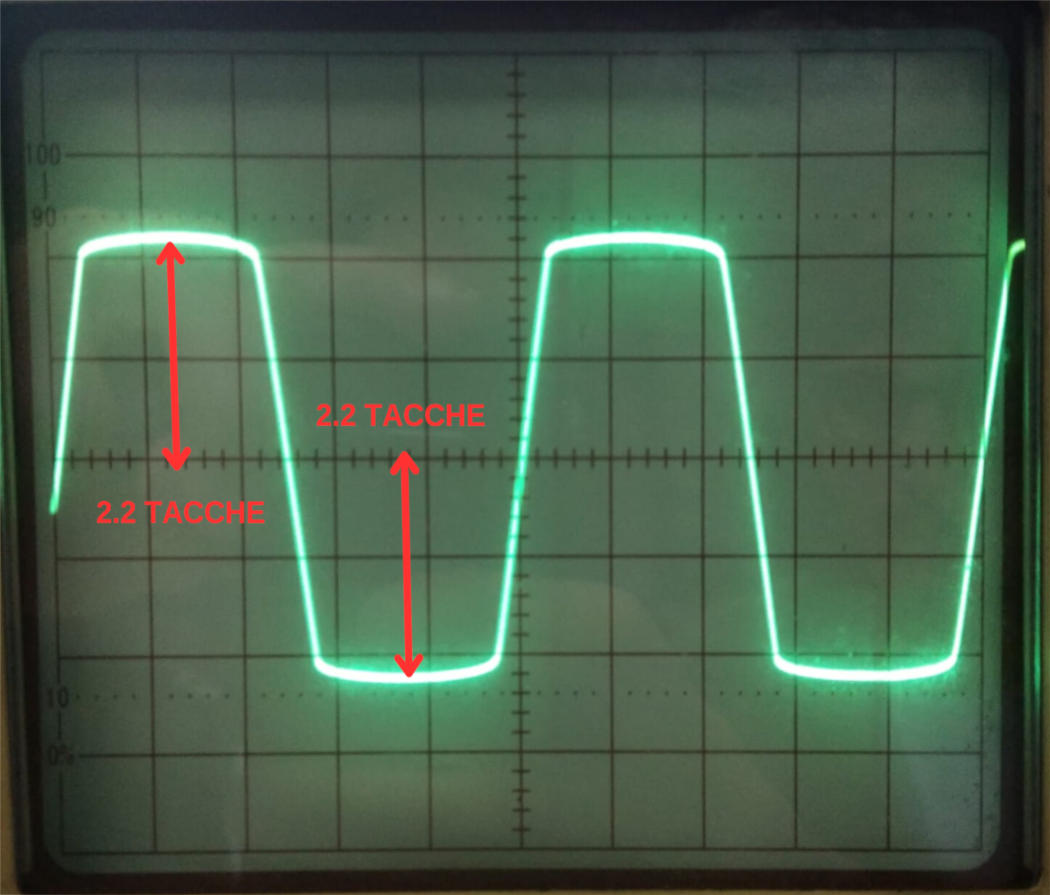
\includegraphics[width=\textwidth]{../assets/Resistenze_Uguali.png}
    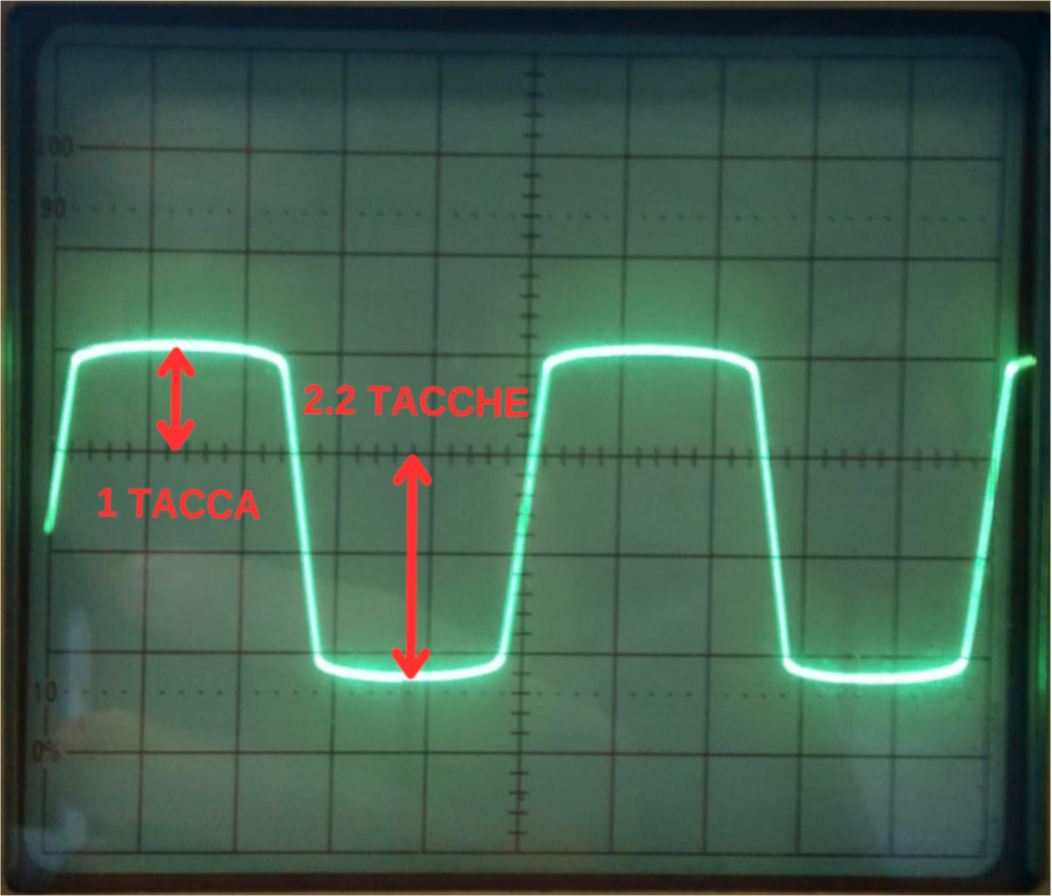
\includegraphics[width=\textwidth]{../assets/Resistenze_Diverse.png}
    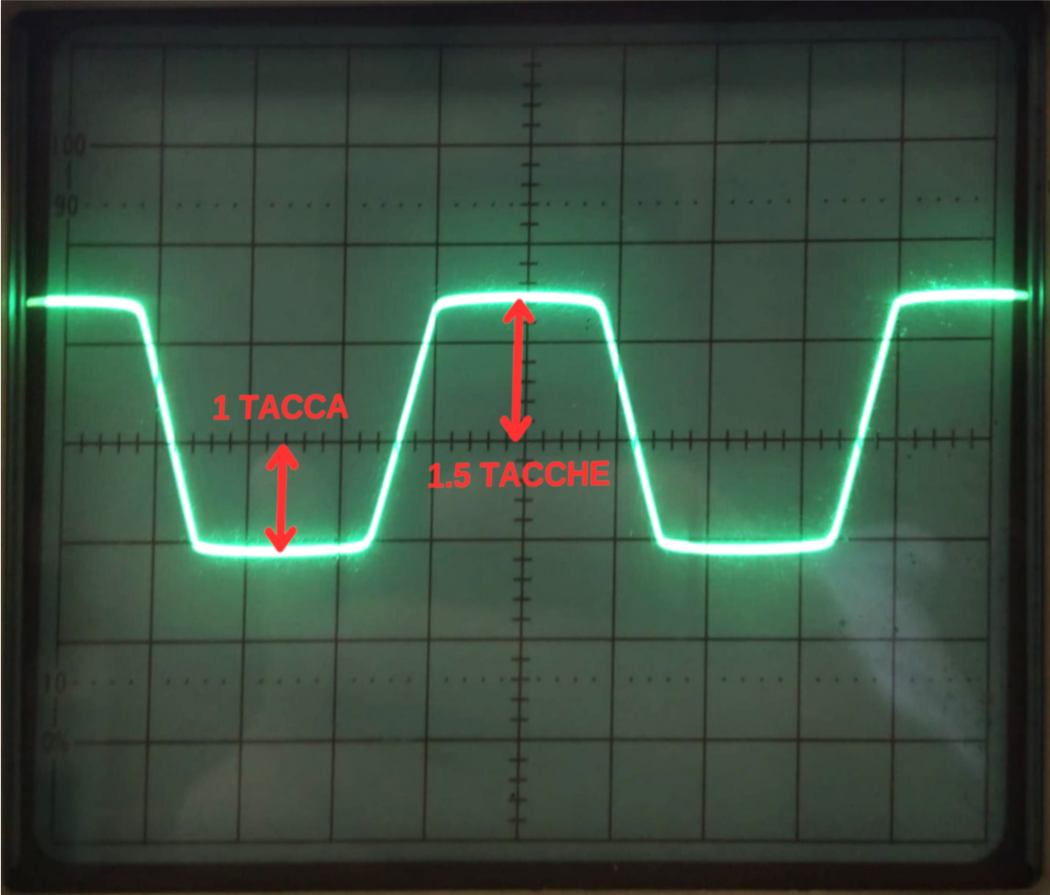
\includegraphics[width=\textwidth]{../assets/Resistenze_Diverse2.png}
    \caption{\emph{Onde quadre generate dal circuito variando i valori delle due resistenze.}}
    \label{fig : dati raccolti}
  \end{figure}